\documentclass[11pt]{scrartcl}
\usepackage[utf8]{inputenc}
\usepackage{mathtools}
\usepackage{amssymb}
\usepackage{listings}
\usepackage{bm}
\usepackage{graphicx}
\lstset
{ %Formatting for code in appendix
	language=Matlab,
	basicstyle=\footnotesize,
	numbers=left,
	stepnumber=1,
	showstringspaces=false,
	tabsize=1,
	breaklines=true,
	breakatwhitespace=false,
}
\begin{document}
\centerline{\LARGE{\textbf{CSE881 HW2}}}
\centerline{\large{\textit{Nan Cao,\  A52871775}}}
\centerline{\large{\textit{Sep 16th, 2016}}}
% \maketitle
\section*{Problem 1}
\textbf{(a)}\\
$x_1$,  generated from a uniform distribution in the range between 0 and 1, is like to produce the same bins regardless of whether using equal width or equal frequency approaches.\\
\textbf{(b)}\\
$x_2$, generated from a mixture 3 normal distributions, is more suitable for equal frequency tan equal width discretization approaches.\\
\textbf{(c)}\\
$x_3$, generated frrom an exponetial distribution, is appropriate for neither equal frequency nor equal width discretization approaches.\\
\textbf{(d)}\\
After discretization, they're all order attributes.
\section*{Problem 2}
\textbf{(a)}\\
\begin{equation*}
\begin{aligned}
A&=[a_{ij}]_{N*d}\\
\frac{1}{N-1} \bm{A}^T[\bm{i}_N- \frac{1}{N}\bm{1}_N]\bm{A}
&=\frac{1}{N-1}{ [\bm{A}- 
[\bar{\bm{a}}_{\cdot j}]_{N*d}]}^T[\bm{A}- 
[\bar{\bm{a}}_{i \cdot}]_{N*d}]\\
&=\frac{1}{N-1} \bm{A}^T{[a_{ij}-\bar{\bm{a}}_{i \cdot}]}_{N*d}\\
&=[\frac{1}{N-1}\sum_{N}^{i=0}(a_{ij}-\bar{\bm{a}}_{i\cdot})]_{N*d}\\
&={\sigma^2_{ij}}_{N*d}=C\\
\end{aligned}
\end{equation*}
\textbf{(b)}\\
\begin{equation*}
\begin{aligned}
(N-1) \bm{X \Lambda X}^T
&=(N-1)\bm{C}\\
&= \bm{A}^T[\bm{I}_N-\frac{1}{N}\bm{1}_N]\bm{A}\\
&= \bm{A}^T \bm{I}_N \bm{A}-\frac{1}{N}\bm{A}^T \bm{1}_N \bm{A}\\
&= \bm{V\Sigma}^2\bm{V}^T
\end{aligned}
\end{equation*}
\textbf{(c)}\\
\begin{equation*}
\begin{aligned}
% \bm{A}_m&=(
% 	 	\bar{\bm{a}}_{\cdot 1},
% 		\bar{\bm{a}}_{\cdot 2},
% 		\bar{\bm{a}}_{\cdot 3},
% 		......,
% 		\bar{\bm{a}}_{\cdot d}
% 		)\\
\bm{A}\ has\ been\ centered\\
\bm{C}=\frac{1}{N-1}\bm{A}^T\bm{A}&=\bm{X \Lambda X}^T\\
(\bm{U }\bm{\Sigma V}^T)^T \bm{U \Sigma V}^T&=\bm{X \Lambda X}^T\\
\bm{V}\bm{\Sigma}^T (\bm{U}^T\bm{U})\bm{\Sigma V}^T&=\bm{X \Lambda X}^T\\
\bm{V}(\bm{\Sigma}^T\bm{\Sigma})\bm{ V}^T&=\bm{X \Lambda X}^T\\
\bm{V}\bm{\Lambda}\bm{V}^T&=\bm{X \Lambda X}^T\\
\bm{V}&=\bm{X}
\end{aligned}
\end{equation*}

\section*{Problem 3}
\textbf{d}
Class of 0 and Class of 1 are easier to be discerned by the first two components and CLasses of 2 and 3 are harder to be discerned?\\
\textbf{e}
Class of 2 and is easier to be discerned.(From my opinion of view, 0 looks similar to 1 and 2 looks similar to 3, if my outcome picture is correct.)\\
\textbf{3f}
Yes, I can visually discern more digit images correctly with the
increasing rank of the matrix W.
\section*{Problem 4}
For digit1, kernel PCA can better discriminate their images than PCA.\\
\\
\LARGE{\textbf{Following are the pictures.}}
\begin{figure} 

	
\includegraphics[width=5.5in,height=3.5in]{digit_image_3b.jpg}
	\caption{Problem 3b}
\end{figure}
\begin{figure} 

	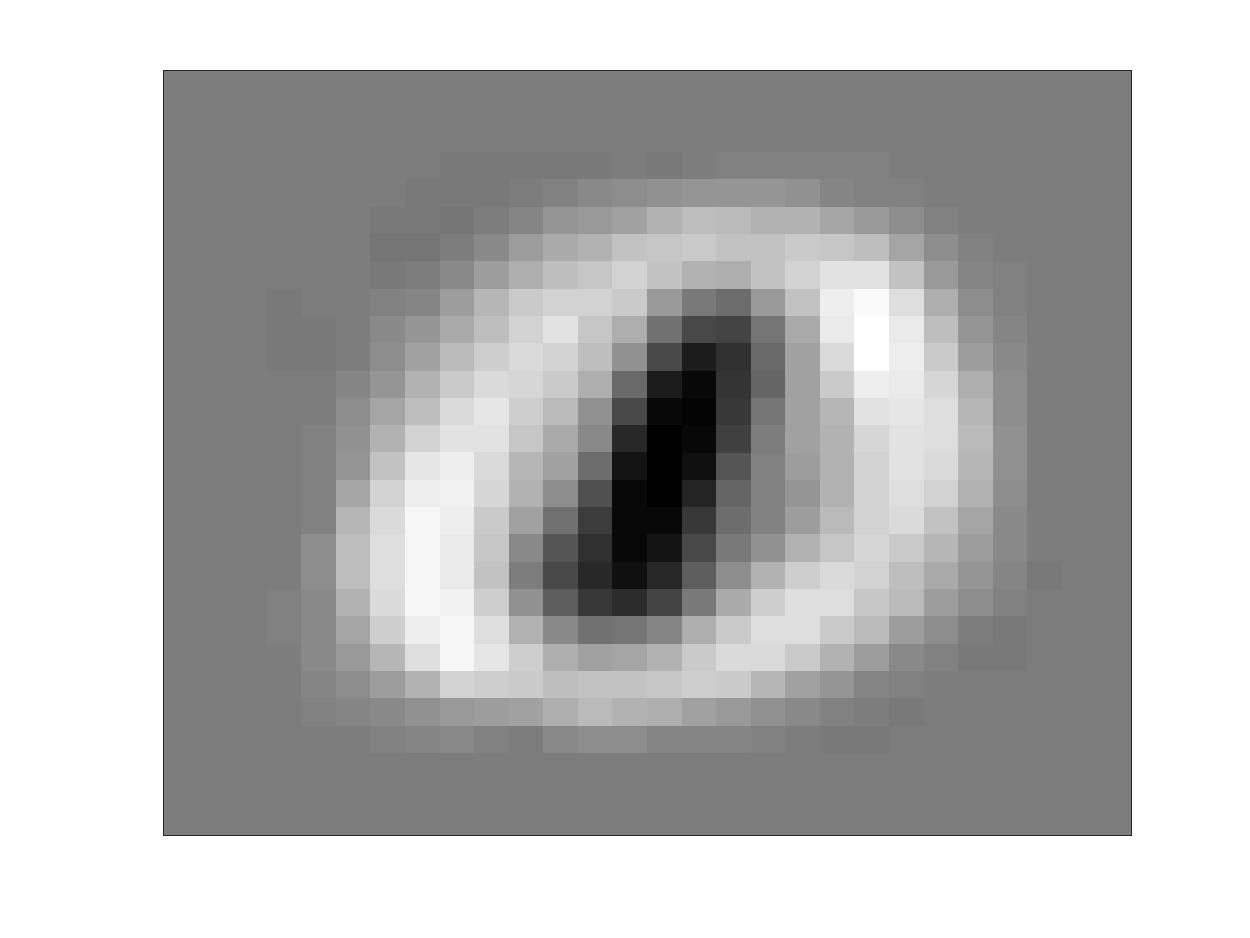
\includegraphics[width=5.5in,height=3.5in]{digit_image_3c1.jpg}
	\caption{Problem 3c-1}
\end{figure}
\begin{figure} 

	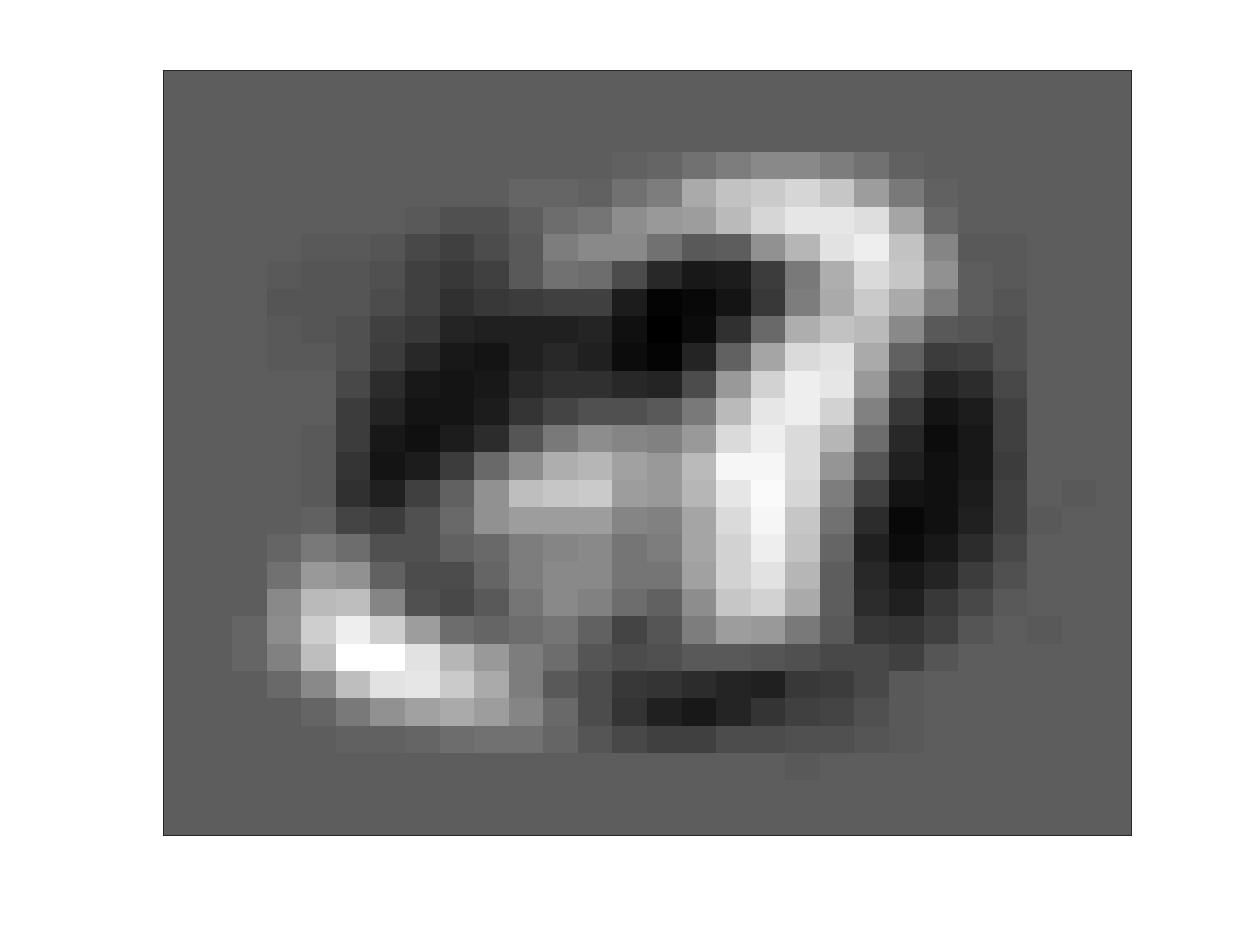
\includegraphics[width=5.5in,height=3.5in]{digit_image_3c2.jpg}
	\caption{Problem 3c-2}
\end{figure}
\begin{figure} 

	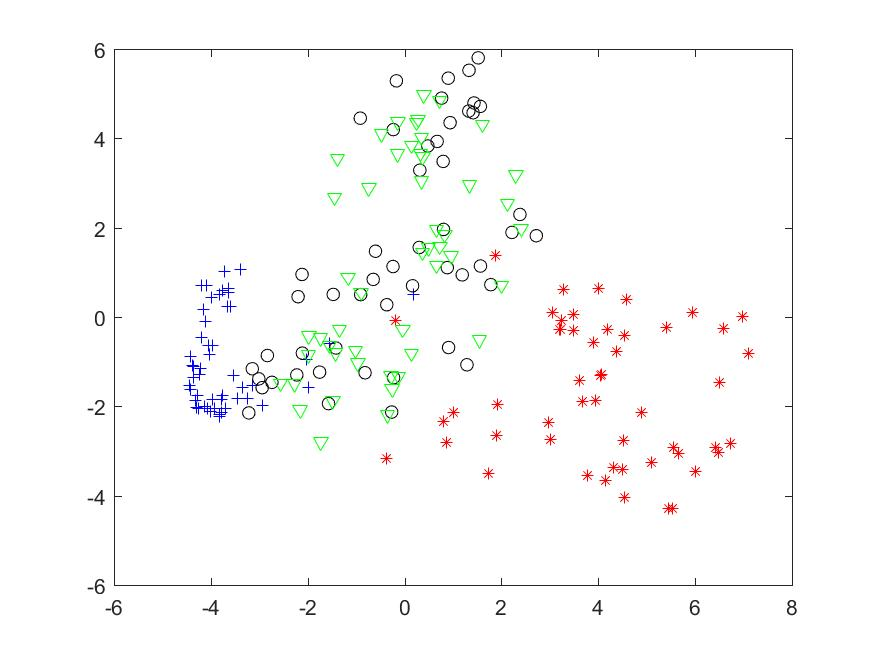
\includegraphics[width=5.5in,height=3.5in]{digit_image_3d.jpg}
	\caption{Problem 3d}
\end{figure}
\begin{figure} 

	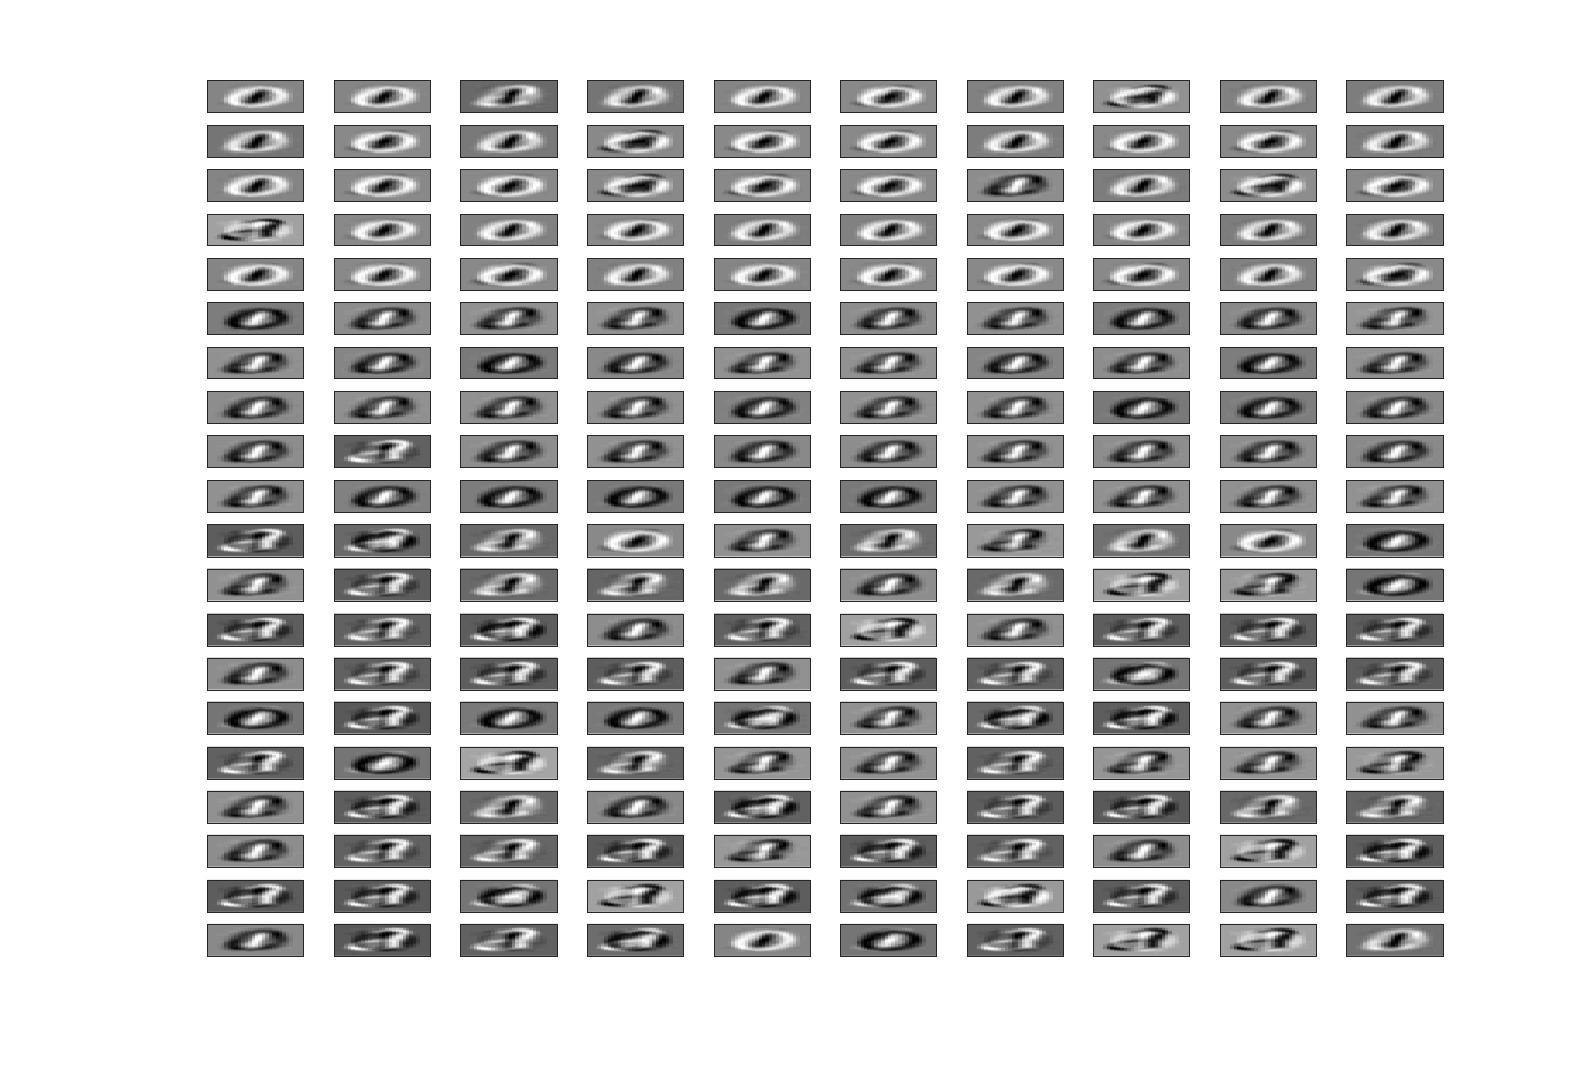
\includegraphics[width=5.5in,height=3.5in]{digit_image_3e.jpg}
	\caption{Problem 3e}
\end{figure}
\begin{figure} 

	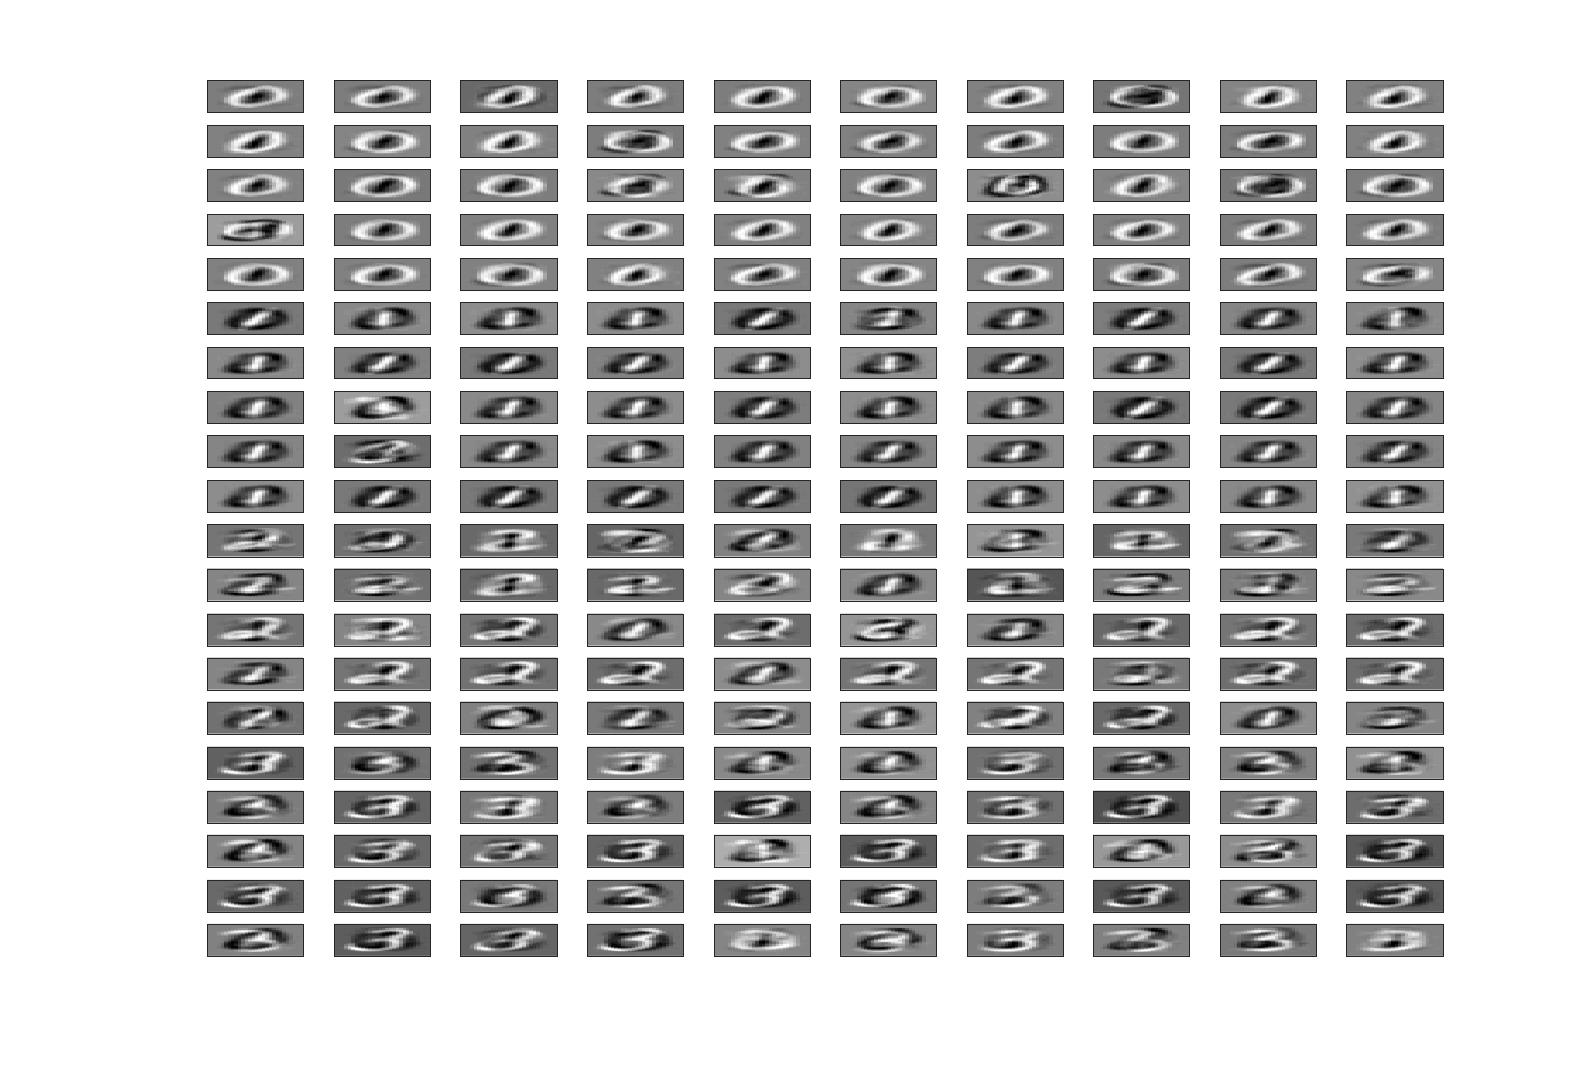
\includegraphics[width=5.5in,height=3.5in]{digit_image_3f.jpg}
	\caption{Problem 3f}
\end{figure}
\begin{figure} 

	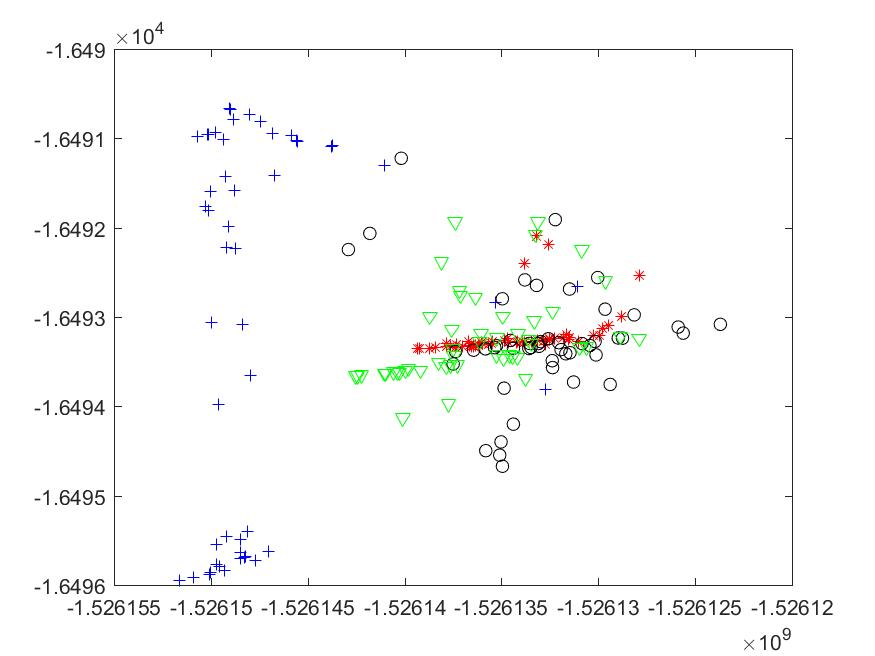
\includegraphics[width=5.5in,height=3.5in]{digit_image_4.jpg}
	\caption{Problem 4 scatter plot}
\end{figure}



\end{document}
% \section*{ProblemX}
% \begin{equation*}
% \begin{aligned}
% \end{aligned}
% \end{equation*}
% \textbf{(a)}\\
% \textbf{(b)}\\
% \textbf{(c)}\\
% \textbf{(d)}\\
% \textbf{(e)}\\
% \textbf{(f)}\\
% \textbf{(g)}\\